\subsubsection{Interaktion}\label{interaktion}

Während des Deployments waren gleichermaßen vollständig durchgeführte Wahl-Interaktionen (Stimmabgabe ist erfolgt) und unvollständige Wahl-Interaktionen (es wurde versucht, eine Stimme abzugeben, aber es gelang nicht) zu beobachten.

Zwei Seniorinnen hielten sich unabhängig von einander für eine Zeit von 30 bis 60 Sekunden in der Wahlkabine auf, ohne dass eine Stimmabgabe erfasst wurde.
Bei einer der beiden Damen war zu beobachten, dass sie sogar in den Korb mit den Wahlkarten griff.
In Folge dessen war für sie entweder unklar, was sie mit den Wahlkarten tun kann oder sie entschloss sich, nicht zu wählen, weil ihre Partei nicht als Wahlkarte abgebildet war (nur als Option ``Sonstige'').

Ein weiterer Passant (ca. Mitte 40) sprach uns aktiv an, als wir uns gerade in der Nähe der Wahlkabine befanden und fragte, ob er dort seine Stimme für die Bundestagswahl abgeben könne.
Nachdem wir ihm das Experiment erklärt hatten, entschloss sich der Mann, an der Umfrage teilzunehmen.
Er löste die mit einer Schnur an der Installation befestigte Wahlkarte (die Befestigung diente dazu, Diebstahl zu verhindern und sollte gleichzeitig verdeutlichen, dass die Wahlkarte wieder zurückzulegen und nicht einzuwerfen ist) und fragte uns, was damit zu tun ist.
Nachdem wir dem Mann das System erklärt hatten, steckte er die Wahlkarte mehrmals hektisch falsch herum in die Wahlurne und war sich im Unklaren darüber, ob seine Stimme erfasst wurde oder nicht.
Der Mann blickte dabei nicht auf das Display, sondern herunter auf die Wahlurne und konnte so auch nach erfolgreicher Stimmabgabe nicht feststellen, dass seine Stimme registriert wurde.
Wir mutmaßen, dass der Mann das Display vollständig ignorierte, weil er glaubte, bereits alle Informationen von uns erhalten zu haben.
Zudem betonte er mehrmals, dass er sehr in Eile ist (der Mann trug erkennbare Arbeitskleidung).
Auch deshalb hat er sich wahrscheinlich nicht noch einmal die Zeit genommen, die Informationen auf dem Display zu lesen.

Um die Interaktion für die ersten Interessenten zu erleichtern, haben wir am Anfang bereits 10 Stimmen hinzugefügt.
Diese waren zufällig, aber entsprechend der Verteilung der damals aktuellen Umfrageergebnisse, gewählt.
Die folgenden Abbildungen zeigen die abgegebenen Stimmen im Zeitverlauf und das Ergebnisse.
Das unbereinigte Ergebnisse entspricht dem, was am Schluss auf Display 1 zu sehen war, und enthält neben den Seed-Daten auch 2 Instanzen von doppelter Stimmabgabe, bei denen jeweils weniger als 10 Sekunden seit der vorhergehenden Teilnahme vergangen waren.
Zusätzlich waren darin Stimmen enthalten, die wir selbst zur Aufzeichnung unseres Videos abgegeben haben.
All diese Stimmen wurden aus dem bereinigten Ergebnis entfernt, das in Abbildung \ref{fig:result-cleaned} zu sehen ist.

\begin{figure}[ht]
    \centering
    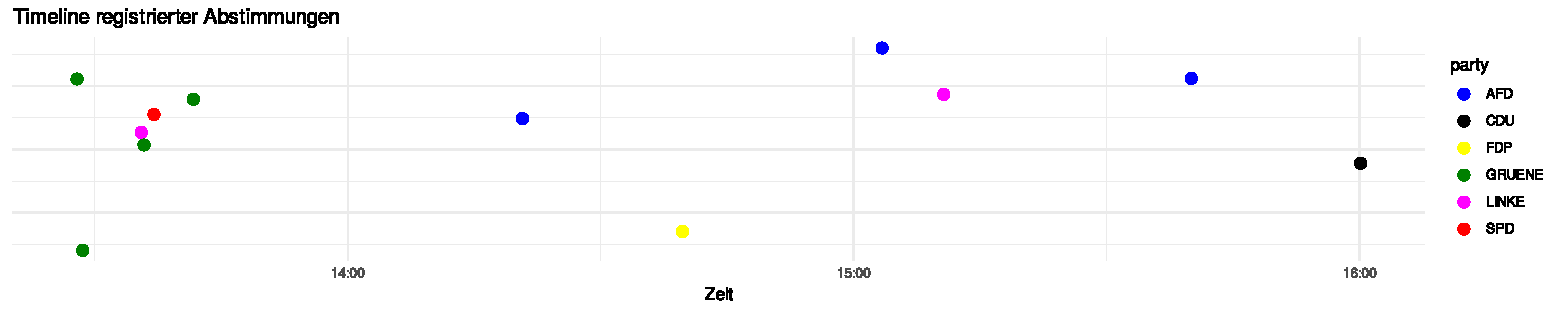
\includegraphics[width=0.8\textwidth]{figures/timeline-cleaned.pdf}
    \caption{Timeline der Interaktionen (bereinigt, siehe Abbildung \ref{fig:result-cleaned})}
    \label{fig:timeline}
\end{figure}

\begin{figure}[ht]
    \centering
    \begin{minipage}{.48\textwidth}
        \centering
        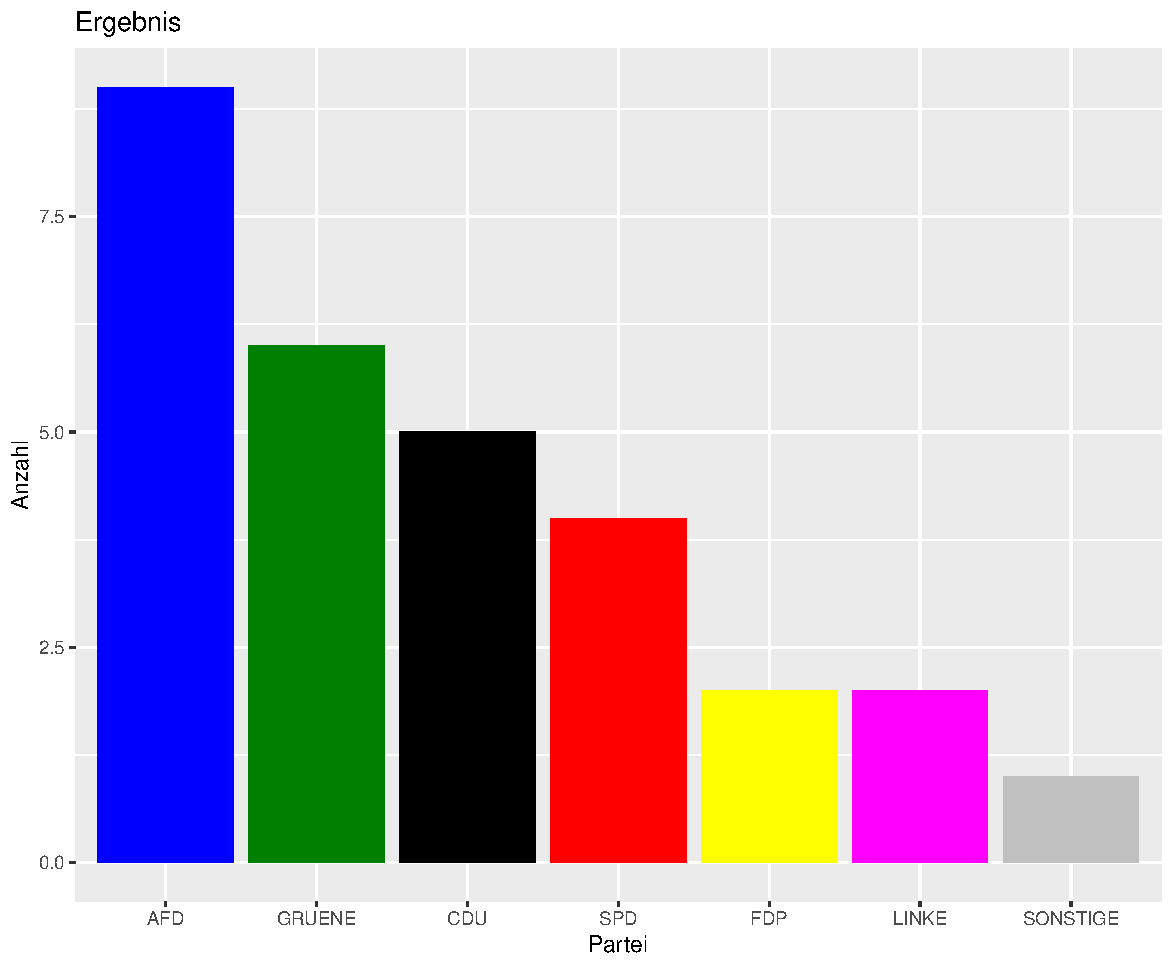
\includegraphics[width=.9\linewidth]{figures/result-all.pdf}
        \captionof{figure}{Abstimmungsergebnis, wie am Ende des Experiments zu sehen}
        \label{fig:result-all}
    \end{minipage}%
    \begin{minipage}{.48\textwidth}
        \centering
        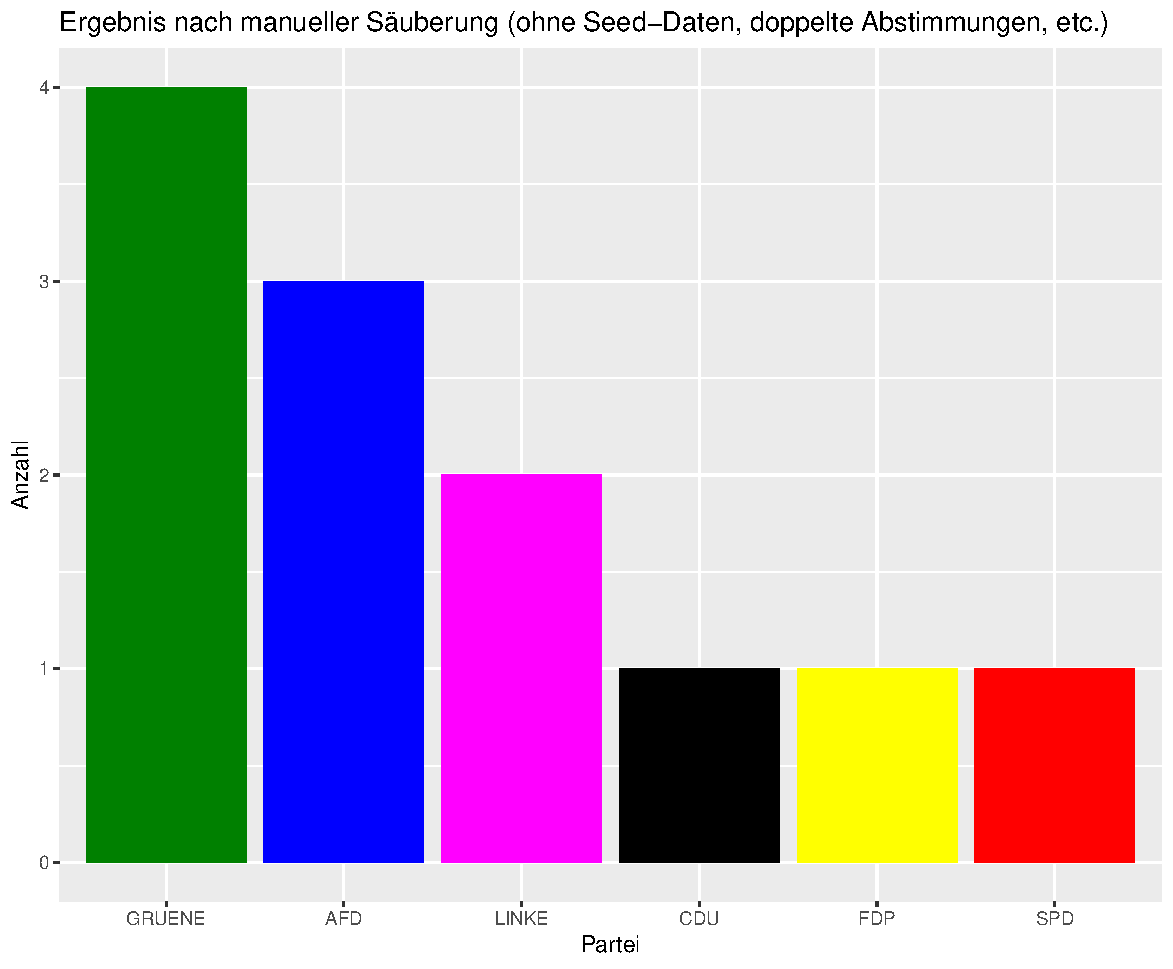
\includegraphics[width=.9\linewidth]{figures/result-cleaned.pdf}
        \captionof{figure}{Abstimmungsergebnis, bereinigt}
        \label{fig:result-cleaned}
    \end{minipage}
\end{figure}